\section{Mobility Platform}\label{sec:platform}

The iRobot PackBot is a fielded small robot used primarily for bomb disposal \cite{iRobot,Hogg2002}. The design is ``semi-modular'' where payloads can be installed to the base chassis, but they can only be installed in specific configurations, and when the software is properly configured. The integration of new payloads is often difficult and expensive. The vehicle uses military BB-2590 Li-Ion rechargeable batteries. While they have been widely deployed to both Iraq and Afghanistan, the PackBot is very expensive to purchase and maintain and overall reliability has been a challenge. There are two different generations: the obsolete 500 version and the current production 510 version. Many parts are interchangeable between the two models. The U.S. Army has discontinued the PackBot and no longer supports it as a program of record.

\begin{figure}
	\centering
	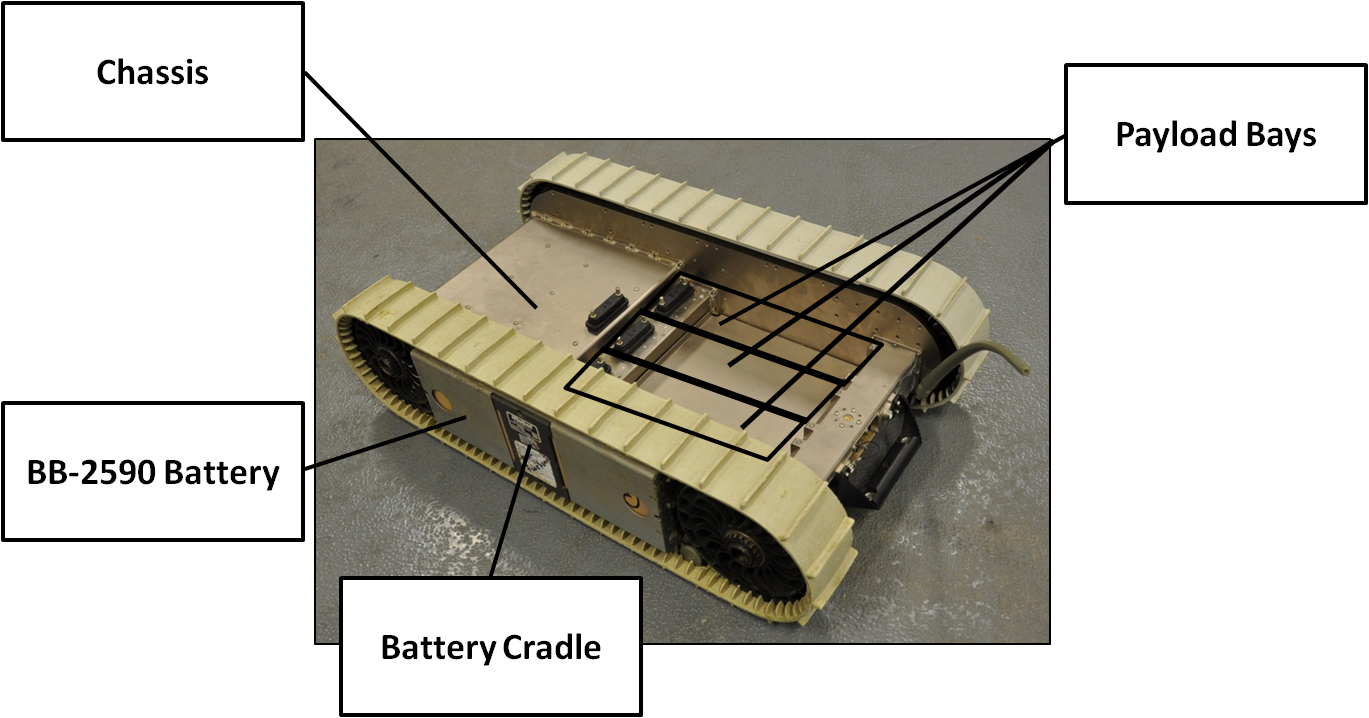
\includegraphics[width=0.48\textwidth]{./pictures/packbot1.png}
	\caption{Anatomy of the GVR-Bot.}
	\label{fig:packbot}
\end{figure}

With a large inventory of unused and unsupported robots, the RS-JPO (Robotic Systems Joint Program Office) funded a 12 month effort to implement IOP (Interoperability Profile V2, using JAUS which is the Joint Architecture for Unmanned Systems) on the existing PackBot platforms. Creating a kit design for retrofitting all fielded PackBots would reduce costs of maintaining the aged fleet. The standardized version of the PackBot makes for a good research platform due to a number of reasons:
\begin{itemize}
	\item Open architecture
	\item Design is completely government-owned
	\item Designed for IOP V1 compliance
	\item Cost is relatively low
\end{itemize}

The research platform became known as the GVR-Bot (Ground Vehicle Robotics is a branch of TARDEC) as shown in Fig.~\ref{fig:packbot}. The radio frequency was changed to 2.4 GHz so it could easily connect over standard and existing wireless Internet protocols. All of the internal electronics of the robot were replaced with new motherboards, interface boards, and motor controllers. Bootloaders were added to the internal control boards, thus allowing all of the software to be flashed without disassembling the robot. See Fig. \ref{fig:pcb} for an example printed circuit board configuration. The internal computer of the GVR-Bot manages linear and rotational accelerations/velocities of the vehicle, odometry, orientation, battery levels, GPS, and communications. The GVR-Bot used for IH missions contains an external embedded computer (Intel Core i7) to perform navigation and obstacle avoidance tasks, video monitoring, sensor integration through a mote (Libelium Waspmote), and collects LiDAR data using a Velodyne HDL-32E.   

\begin{figure}[b]
	\centering
	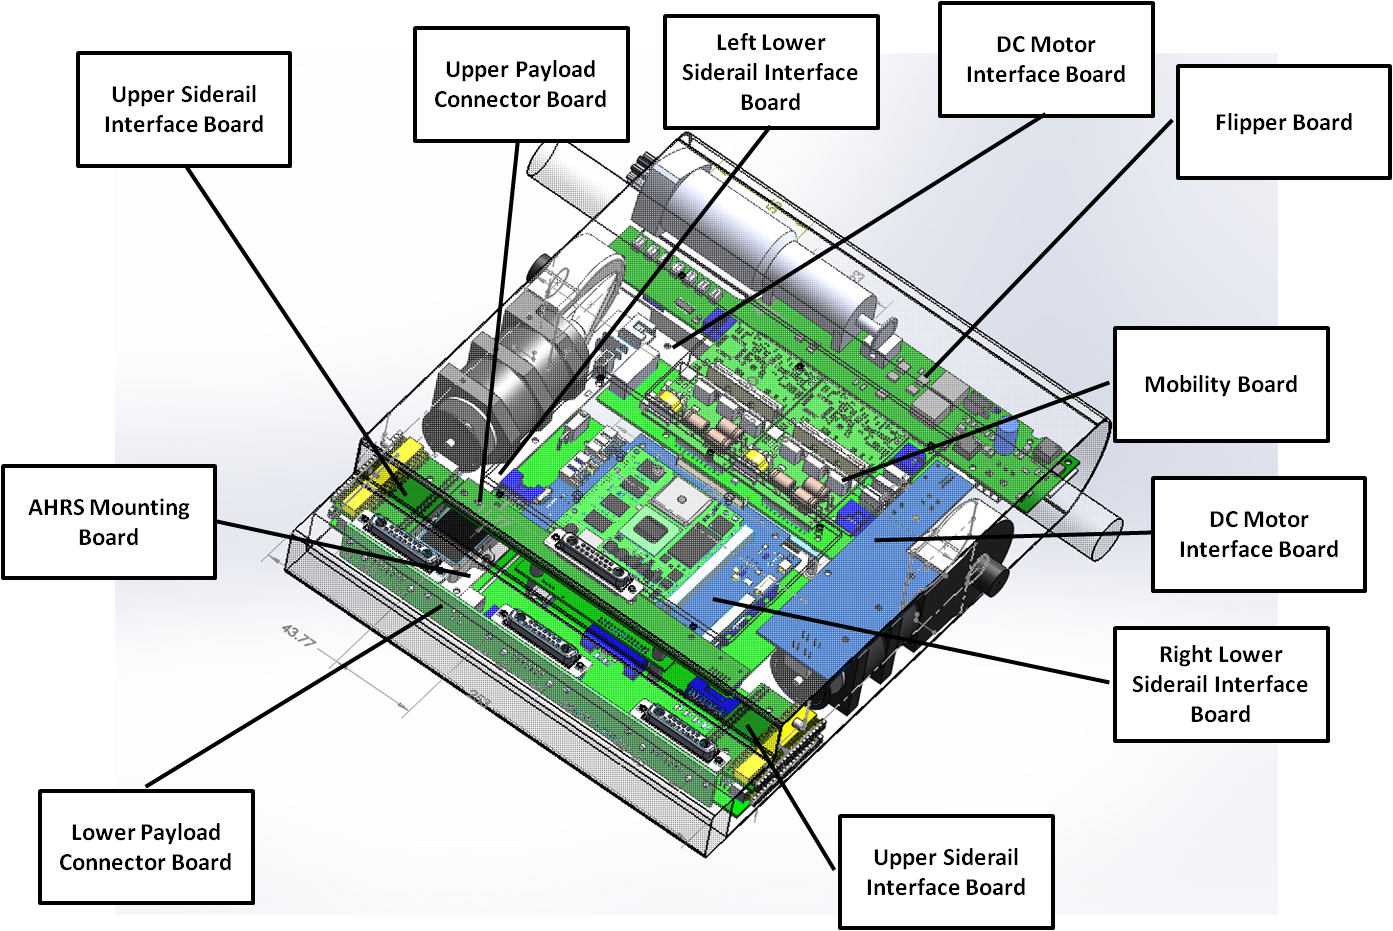
\includegraphics[width=0.48\textwidth]{./pictures/pcb.png}
	\caption{Front assembly interface board. This printed circuit board and sub-assemblies are part of the complete electrical component redesign of the Packbot.}
	\label{fig:pcb}
\end{figure}

%  Add in stuff about lidar and how it moves up and down (pitches on Y) or yaws 180deg on Z (sweeping back-forth) sitting on its side 
%what about the kind of processing power it has on-board to do this slam crap 
